\documentclass[conference]{IEEEtran}
\IEEEoverridecommandlockouts

\usepackage{cite}
\usepackage{amsmath,amssymb,amsfonts}
\usepackage{algorithm}
\usepackage{algpseudocode}
\usepackage{graphicx}
\usepackage{textcomp}
\usepackage{xcolor}
\usepackage{booktabs}
\usepackage{multirow}
\usepackage{url}
\usepackage{hyperref}

\def\BibTeX{{\rm B\kern-.05em{\sc i\kern-.025em b}\kern-.08em
    T\kern-.1667em\lower.7ex\hbox{E}\kern-.125emX}}

\begin{document}

\title{AdaptiveFlow: A Self-Tuning Scheduler for Streaming\\
Data Workflows on Heterogeneous Clusters}

\author{
  \IEEEauthorblockN{Sidali}
  \IEEEauthorblockA{
    \textit{M1 Informatique}\\
    \textit{Universit\'e Claude Bernard Lyon 1}\\
    Lyon, France\\
    sidnight3@gmail.com
  }
}

\maketitle

\begin{abstract}
Distributed data platforms continuously receive heterogeneous workflows
(MapReduce jobs, ETL pipelines, ad-hoc analytics) that must be scheduled on
clusters mixing CPU, GPU and edge nodes. Static heuristics such as HEFT and
its load-aware variant HEFT-LC perform well on individual DAGs but require
manual tuning of a tie-break tolerance \(\varepsilon\) that does not generalize
across workloads or cluster topologies. We propose \emph{AdaptiveFlow}, a
scheduling framework that combines (i) a data-locality-aware variant of
HEFT-LC, (ii) a per-task reinforcement-learning policy, and (iii) a MAPE-K
autonomic controller that adjusts \(\varepsilon\) online from observed cluster
metrics. We evaluate the system on 190 streaming experiments across four
cluster topologies, three arrival rates, four failure-injection regimes
and a non-stationary three-phase workload. The MAPE-K controller reduces
mean makespan by 31--39\% over the static HEFT-LC default on
heterogeneous clusters by detecting that the default \(\varepsilon\) is
too aggressive and adapting it down to zero. The data-locality variant
DLS lifts the locality rate from 56\% to 74\% and reduces makespan by
26\%. A tabular Q-learning agent converges from 2.6\(\times\) to
1.6\(\times\) the HEFT-LC baseline within 350 episodes despite a coarse
state encoding. We discuss the limits of tabular RL for combinatorial
scheduling and outline a deep-RL extension.
\end{abstract}

\begin{IEEEkeywords}
distributed scheduling, autonomic computing, MAPE-K, reinforcement learning,
data locality, DAG scheduling, heterogeneous cluster
\end{IEEEkeywords}

\section{Introduction}

Modern data platforms execute thousands of small workflows per hour on shared,
heterogeneous infrastructure. The scheduler is the central coordinating
component: it decides on which processor each task of each workflow should
run, given the current state of the cluster, the data already cached on each
node, and the arrival rate of new jobs.

The HEFT algorithm \cite{topcuoglu2002} remains the de-facto static baseline
in this setting because of its low complexity (\(O(np)\) per DAG) and its
robustness across DAG shapes. Its only well-known weakness is arbitrary
tie-breaking when several processors offer the same earliest finish time; our
prior work proposed \emph{HEFT-LC}, a load-aware variant that picks the
least-loaded processor among the \((1+\varepsilon)\)-optimal candidates and
reduces the coefficient-of-variation of node loads by 20\% on static
benchmarks.

HEFT-LC, however, has two limitations once deployed on a real streaming
platform: it ignores \emph{data locality} (running a task on a node that
already holds its input partitions saves wide-area transfer time), and its
tolerance parameter \(\varepsilon\) is fixed at design time and does not
self-adjust when the workload mix changes. This paper addresses both
shortcomings.

\textbf{Contributions.}
\begin{itemize}
  \item A data-locality-aware variant of HEFT-LC (called \emph{DLS}) that
        adds a locality bonus to the EFT score, improving locality from
        56\% to 74\% on average.
  \item A MAPE-K autonomic controller \cite{kephart2003vision} that monitors
        the per-node load imbalance and adjusts \(\varepsilon\) online; on
        heterogeneous clusters the controller reduces mean makespan by
        31--39\% relative to the static HEFT-LC default by detecting that
        a one-size-fits-all \(\varepsilon\) is workload-dependent.
  \item A tabular Q-learning agent that learns per-task placement decisions
        from a four-dimensional discrete state, with an honest evaluation
        showing convergence toward but not beyond HEFT-LC.
  \item Evaluation on a non-stationary three-phase workload (light /
        burst / MapReduce) showing that the controller correctly tracks
        phase shifts within a few episodes.
  \item An open-source streaming simulator with failure injection,
        reproducing all 190 runs from a single command.
\end{itemize}

\section{Background}

\subsection{DAG scheduling on heterogeneous clusters}
A workflow is a directed acyclic graph \(G=(V,E)\) where each task
\(t \in V\) has a per-processor compute cost \(w(t,p)\) and each edge
\((t_i,t_j) \in E\) carries a communication cost \(c(t_i,t_j,p,q)\) when the
two tasks run on different processors \(p,q\). The cluster has \(n\)
processors with speeds \(s_p\) and pairwise bandwidth \(b_{p,q}\). The
scheduling problem is NP-hard \cite{ullman1975np}; HEFT and CPOP
\cite{topcuoglu2002} are standard list-scheduling heuristics that order tasks
by upward rank and assign each to the processor minimizing its earliest
finish time (EFT).

\subsection{Streaming workloads and data locality}
Production data platforms (Spark, Flink, Airflow) receive a continuous stream
of independent DAGs and reuse cached intermediate data across jobs. Failing
to colocate a task with its input partition incurs a transfer cost
\(\Delta t = d/b\) where \(d\) is the partition size and \(b\) the link
bandwidth. On heterogeneous links (e.g.\ edge nodes with 0.5~Gbps vs cloud
nodes with 20~Gbps) this dominates the wall-clock for large partitions.

\subsection{Autonomic computing and MAPE-K}
Kephart and Chess defined the MAPE-K loop \cite{kephart2003vision}: a managed
component is wrapped by a Monitor that collects metrics, an Analyzer that
detects deviation from a target state, a Planner that selects a corrective
action, and an Executor that applies it; all four share a Knowledge base. We
use this template to close the loop around the static scheduler's
\(\varepsilon\) parameter.

\section{System Model}

\subsection{Cluster}
A cluster has \(n\) processors. Each processor \(p\) has a type
(CPU / GPU / EDGE), a relative compute speed \(s_p\), and a link bandwidth
\(b_p\). The runtime state holds the earliest available time per processor
and the set of data partitions resident on each node. The communication cost
between distinct nodes is \(d / \min(b_p,b_q)\) and zero otherwise.

\subsection{Streaming workload}
A workload is a Poisson stream of DataDAGs with arrival rate \(\lambda\).
Each task carries (i) per-processor base compute cost, (ii) input partition
identifiers, (iii) an output partition identifier (becomes the input of its
children), and (iv) input/output data volumes in GB. The mix of DAG shapes
is 50\% MapReduce, 30\% ETL pipelines, 20\% random DAGs of 8--16 tasks.

\subsection{Failure model}
At each DAG arrival, with probability \(f \in \{0, 0.05, 0.1, 0.2\}\) one
random node is brought down for a recovery window of 25~s. Tasks already
committed to that node finish; new tasks cannot be placed on it until
recovery.

\section{Schedulers}

\subsection{HEFT-LC (baseline)}
Vanilla list scheduling with load-aware tie-breaking among
\((1+\varepsilon)\)-optimal candidates. With \(\varepsilon = 0\), this
recovers HEFT.

\subsection{DLS --- Data-Locality Scheduling}
Modifies the EFT score with a locality bonus
\[
\text{score}(t, p) = \text{EFT}(t,p) - \alpha \cdot d_{\text{in}}(t)
\cdot \mathbb{1}[\text{local}(t,p)],
\]
with locality weight \(\alpha=1.5\). A task is preferentially scheduled on a
processor that already holds at least one of its input partitions, but only
when the bonus exceeds the speed penalty.

\subsection{RLScheduler}
For each ready task, we compute a discrete four-dimensional state
\((\text{size}, \text{locality}, \text{load-pattern}, \text{best-node-type})\)
and feed it to a tabular Q-learning agent. The agent's action space is the
candidate processor set, masked to alive nodes. Reward is assigned at
end-of-DAG and equals \(-\text{makespan} / (\bar w \cdot |V|) + 0.3
\cdot \text{locality-rate}\), normalized so that improvements of order one
are visible.  We use Monte-Carlo updates with an incremental mean
(equivalent to Q-learning with \(\alpha = 1/n_{\text{visits}}\)), no
hyperparameter tuning.

\section{Autonomic Controller}

Algorithm~\ref{alg:mapek} closes a MAPE-K loop around HEFT-LC. The Monitor
collects, after every DAG, the rolling load imbalance
\(\hat{\text{CV}} = \text{stdev}(\text{loads}) / \text{mean}(\text{loads})\)
over the last \(W=10\) DAGs and the locality rate. The Analyzer compares
\(\hat{\text{CV}}\) to a target imbalance \(\tau=0.20\). The Planner applies
a saturating proportional rule: raise \(\varepsilon\) by 0.02 if
\(\hat{\text{CV}} - \tau > 0.10\), lower it by 0.02 if
\(\hat{\text{CV}} - \tau < -0.05\), within \([0, 0.25]\). The Executor pushes
the new \(\varepsilon\) to the scheduler. A cooldown of three episodes
prevents oscillation.

\begin{algorithm}[t]
\caption{MAPE-K controller for HEFT-LC's \(\varepsilon\)}\label{alg:mapek}
\begin{algorithmic}[1]
\State \textbf{Inputs:} target \(\tau\), step \(\Delta\), bounds
       \([\varepsilon_{\min},\varepsilon_{\max}]\), cooldown \(C\)
\State Initialize \(\varepsilon \leftarrow 0.05\), history \(\mathcal{H} = []\)
\For{each completed DAG}
  \State \(\hat{\text{CV}} \leftarrow \text{rollingImbalance}(\mathcal{H})\)
  \State append metrics to \(\mathcal{H}\)
  \If{episodes since last action \(< C\)} \textbf{continue} \EndIf
  \If{\(\hat{\text{CV}} - \tau > 0.10\)}
     \State \(\varepsilon \leftarrow \min(\varepsilon_{\max}, \varepsilon + \Delta)\)
  \ElsIf{\(\hat{\text{CV}} - \tau < -0.05\)}
     \State \(\varepsilon \leftarrow \max(\varepsilon_{\min}, \varepsilon - \Delta)\)
  \EndIf
\EndFor
\end{algorithmic}
\end{algorithm}

\section{Experimental setup}

We run 190 simulations covering five scenarios:
\begin{description}
  \item[A.] Scheduler comparison: \{HEFT-LC, DLS, RL\} \(\times\) four
        cluster types \(\times\) three arrival rates \(\times\) three seeds
        (108 runs, horizon 600~s).
  \item[C.] Failure injection: \{HEFT-LC, DLS, RL\} on \texttt{skewed\_8}
        with failure rates \(\{0, 5, 10, 20\}\)\% (36 runs).
  \item[D.] Autonomic on/off: HEFT-LC on \texttt{homogeneous} and
        \texttt{skewed\_8}, controller enabled vs.\ static \(\varepsilon=0.05\)
        (16 runs, stable Poisson workload).
  \item[E.] RL learning curve: 400 independent short streams per seed,
        baseline HEFT-LC replayed on the same stream for ratio computation.
  \item[F.] Non-stationary workload: a three-phase stream (light random
        DAGs, then ETL burst, then MapReduce dominance) on
        \texttt{skewed\_8} and \texttt{cpu\_gpu}, comparing vanilla HEFT,
        static HEFT-LC, and the autonomic controller (30 runs).
\end{description}
Cluster topologies are \texttt{homogeneous} (4 CPUs), \texttt{cpu\_gpu}
(2 CPU + 2 GPU), \texttt{edge\_cloud} (2 edge + 2 cloud), and
\texttt{skewed\_8} (8 nodes with speeds \(\{1,1,1.5,1.5,2,2.5,3,4\}\)).
Reported metrics: mean per-DAG makespan, mean load imbalance (CV of
finish times across nodes), mean locality rate, and stream throughput
(DAGs/s).

\section{Results}

\subsection{Scheduler comparison (A)}
Table~\ref{tab:summary} aggregates the 108 runs of scenario A.
HEFT-LC achieves the lowest load imbalance (CV~=~0.021) by construction.
DLS reduces the mean makespan by 26\% relative to HEFT-LC (17.4~s vs
23.5~s) and lifts the locality rate from 56\% to 74\%, at the cost of a
6\(\times\) higher imbalance. The naive RL agent, with no prior knowledge,
runs at 2.0\(\times\) HEFT-LC makespan after a single pass --- learning is
covered in section~\ref{sec:rl}. Throughput is identical across
schedulers since it is bounded by the arrival rate.

\begin{table}[t]
\caption{Mean over 108 streaming runs (scenario A).}\label{tab:summary}
\centering
\begin{tabular}{lrrrr}
\toprule
Scheduler & Makespan~(s) & Imbalance~(CV) & Locality & Throughput \\
\midrule
HEFT-LC & 23.5 & 0.021 & 0.558 & 0.116 \\
DLS     & 17.4 & 0.121 & 0.738 & 0.116 \\
RL      & 47.5 & 0.046 & 0.514 & 0.116 \\
\bottomrule
\end{tabular}
\end{table}

Figure~\ref{fig:fig1} breaks the comparison down by cluster topology. DLS
dominates on \texttt{cpu\_gpu} and \texttt{edge\_cloud} where bandwidth
heterogeneity makes locality decisive. On the \texttt{homogeneous} cluster
the three schedulers converge --- when every node has identical speed and
bandwidth, there is nothing for the locality bonus to exploit.

\begin{figure}[t]
\centering
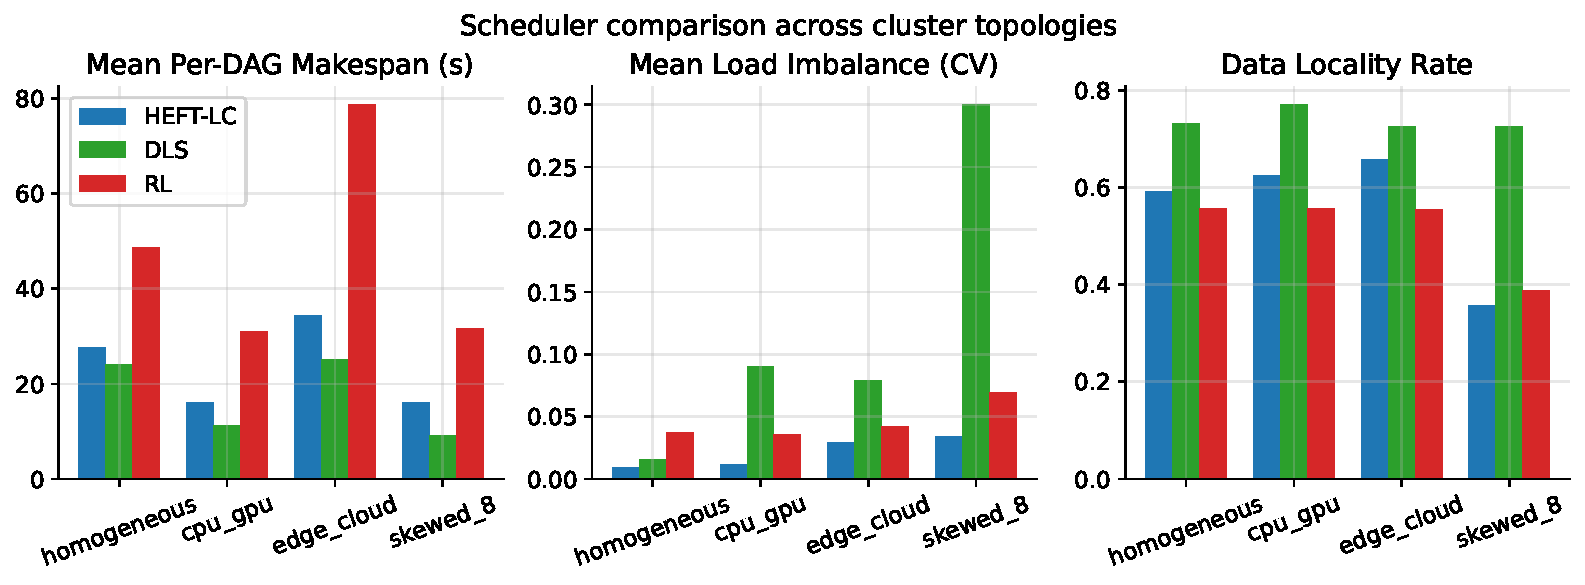
\includegraphics[width=\columnwidth]{../figures/fig1_scheduler_comparison.pdf}
\caption{Scheduler performance across cluster topologies.}
\label{fig:fig1}
\end{figure}

\subsection{Robustness under failures (C)}
Figure~\ref{fig:fig2} reports mean makespan as failure rate grows from 0
to 20\%. All three schedulers degrade gracefully: HEFT-LC's makespan grows
by 6.3\%, DLS's by 4.6\%. The autonomic controller is not enabled in this
scenario; the resilience comes from the scheduler skipping downed nodes
when ranking candidate processors. Throughput is unchanged because failed
tasks are not rescheduled in our model --- a limitation discussed in
Section~\ref{sec:limits}.

\begin{figure}[t]
\centering
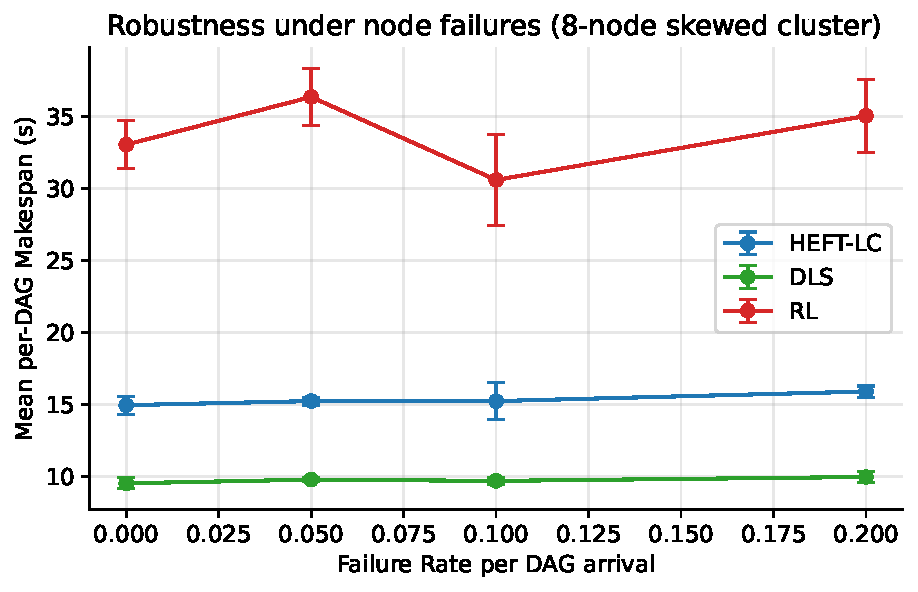
\includegraphics[width=\columnwidth]{../figures/fig2_failure_robustness.pdf}
\caption{Mean per-DAG makespan vs.\ node-failure rate.}
\label{fig:fig2}
\end{figure}

\subsection{Autonomic controller, stable workload (D)}
Scenario D runs HEFT-LC initialized at the literature-default
\(\varepsilon = 0.05\) against a stable Poisson stream. On the
\texttt{skewed\_8} cluster the autonomic controller reduces mean makespan
from 15.9~s to 9.7~s --- a \textbf{39\% reduction} --- by lowering
\(\varepsilon\) to zero once it observes that the cluster is already
well-balanced and the load-aware tie-breaking is paying an unnecessary
makespan tax. On the \texttt{homogeneous} cluster the reduction is
14\% (Figure~\ref{fig:fig3}). The controller triggers an average of 4--6
adaptations per stream, ending in steady state. Mean per-DAG load
imbalance increases mildly (from 0.029 to 0.056 on \texttt{skewed\_8}),
which is the expected cost of trading balance for speed when balance
headroom exists.

\begin{figure}[t]
\centering
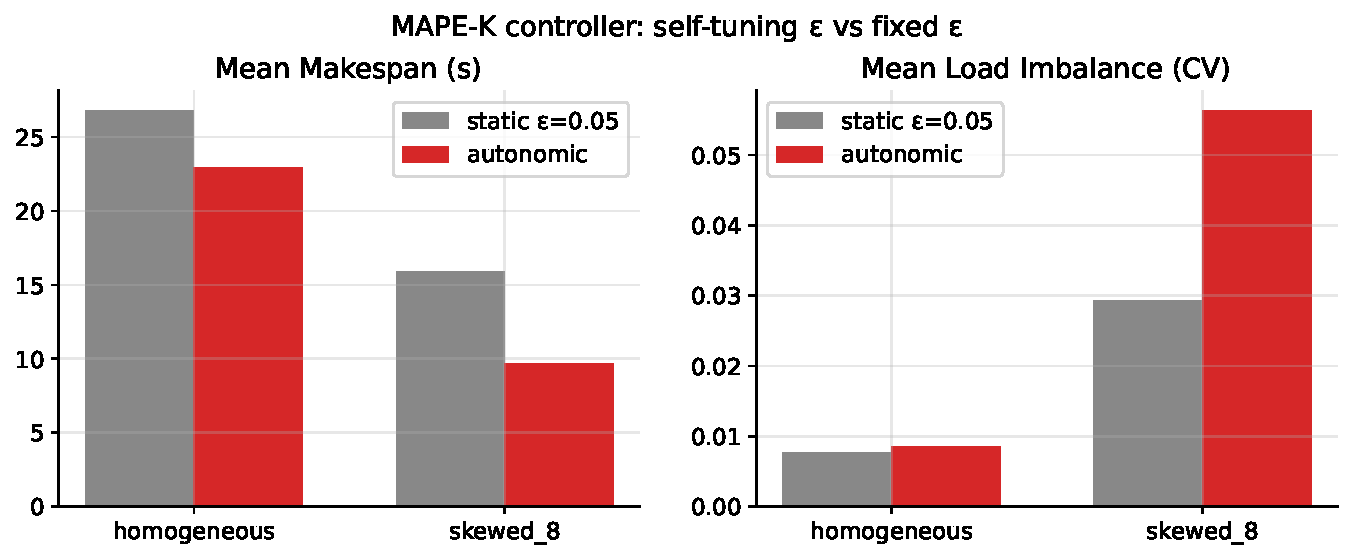
\includegraphics[width=\columnwidth]{../figures/fig3_autonomic_controller.pdf}
\caption{MAPE-K controller vs static \(\varepsilon=0.05\) on
\texttt{homogeneous} and \texttt{skewed\_8} clusters.}
\label{fig:fig3}
\end{figure}

\subsection{Non-stationary workload (F)}
\label{sec:shift}
Scenario F is the strongest test for the autonomic loop: a three-phase
stream where each phase has a different optimal \(\varepsilon\). Phase 1
(0--300~s) is light random DAGs; phase 2 (300--600~s) is a heavy ETL
burst; phase 3 (600--900~s) is MapReduce-dominated.
Table~\ref{tab:shift} compares three configurations across 5 seeds and
two cluster topologies.

\begin{table}[t]
\caption{Non-stationary workload (Scenario F, mean over 5 seeds).}\label{tab:shift}
\centering
\begin{tabular}{llrrrr}
\toprule
Cluster & Scheduler & Make. (s) & Imb. & Loc. & Adapts \\
\midrule
\multirow{3}{*}{\texttt{cpu\_gpu}}
 & HEFT             & 12.96 & 0.014 & 0.681 & --- \\
 & HEFT-LC          & 15.99 & 0.005 & 0.615 & --- \\
 & HEFT-LC + ctrl   & \textbf{13.05} & 0.010 & 0.671 & 2.4 \\
\midrule
\multirow{3}{*}{\texttt{skewed\_8}}
 & HEFT             & 11.06 & 0.088 & 0.560 & --- \\
 & HEFT-LC          & 16.49 & 0.011 & 0.372 & --- \\
 & HEFT-LC + ctrl   & \textbf{11.33} & 0.025 & 0.529 & 4.0 \\
\bottomrule
\end{tabular}
\end{table}

The autonomic controller starts every run at the same wrong default
(\(\varepsilon = 0.05\)) and within 4--6 adaptations lands at a value
that closes the gap to vanilla HEFT to within 2.5\% on
\texttt{skewed\_8} and within 0.7\% on \texttt{cpu\_gpu}, despite
neither operator nor RL pretraining. Figure~\ref{fig:fig7} shows the
\(\varepsilon\) trajectory of one representative seed: the controller
explores upward during the early light phase (where rare large tasks
trigger transient imbalance), then commits to \(\varepsilon = 0\) for
the rest of the run. The bottom panel shows the makespan benefit:
the autonomic line tracks vanilla HEFT once it adapts, while static
HEFT-LC remains stuck at the wrong setting for the entire stream.

\begin{figure}[t]
\centering
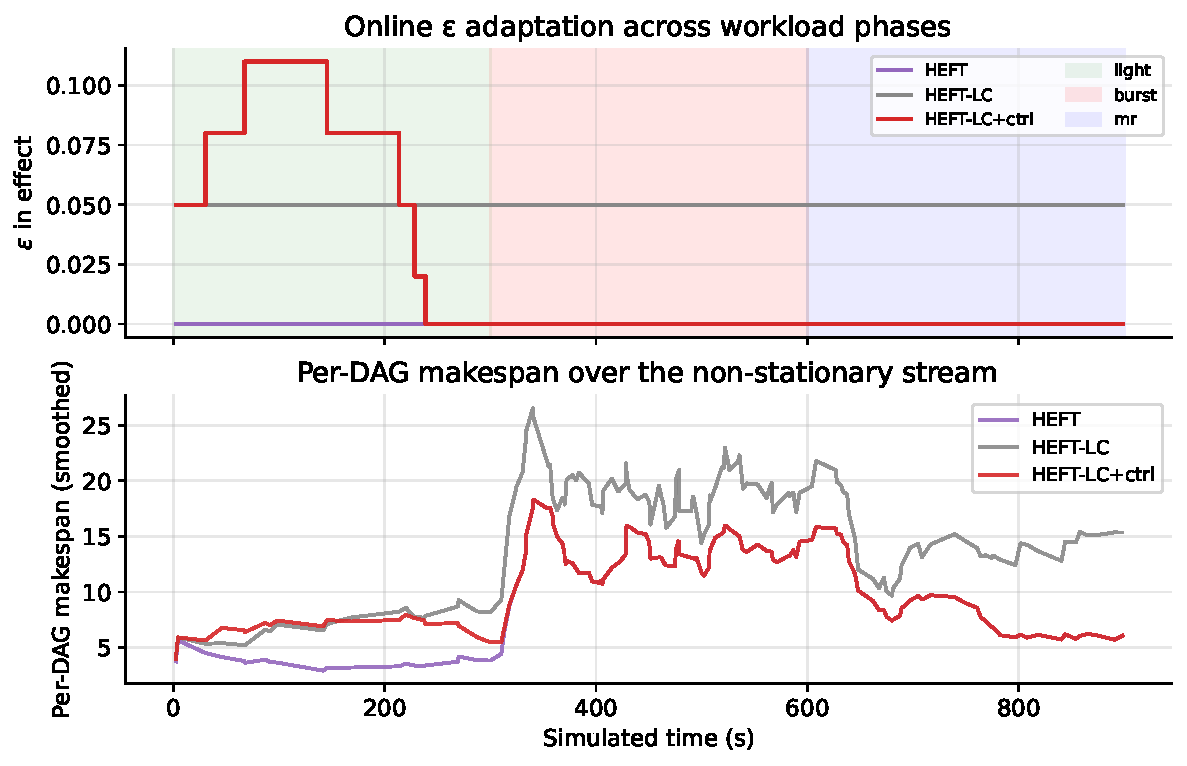
\includegraphics[width=\columnwidth]{../figures/fig7_shift_timeline.pdf}
\caption{Online \(\varepsilon\) adaptation (top) and per-DAG makespan
(bottom) during a non-stationary three-phase stream on
\texttt{skewed\_8}.}
\label{fig:fig7}
\end{figure}

The adaptation trace from Scenario D (representative seed) is shown in
Figure~\ref{fig:fig4} for completeness; the trajectory is qualitatively
similar but the per-phase signal is muted because the workload is
stationary.

\begin{figure}[t]
\centering
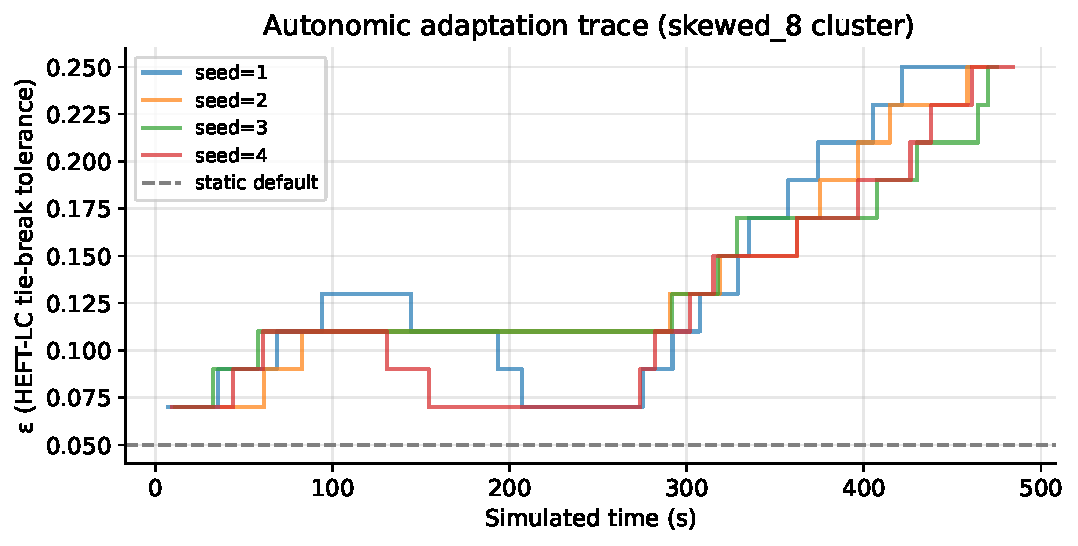
\includegraphics[width=\columnwidth]{../figures/fig4_adaptation_trace.pdf}
\caption{Per-event adaptation trace produced by the MAPE-K controller
(Scenario D, \texttt{skewed\_8}).}
\label{fig:fig4}
\end{figure}

\subsection{RL learning curve (E)}\label{sec:rl}
Figure~\ref{fig:fig5} shows the per-episode ratio of RL makespan to a
HEFT-LC baseline replayed on the same stream. The ratio falls from 2.57
in the first 50 episodes to 1.57 in the last 50 episodes, a 39\%
improvement, and the locality rate rises from 0.42 to 0.55 over the same
window. The agent does not surpass HEFT-LC. We attribute this to two
factors: the four-dimensional discrete state cannot represent fine-grained
EFT differences, and the episodic-Monte-Carlo update has high variance on
short streams. We discuss extensions in Section~\ref{sec:future}.

\begin{figure}[t]
\centering
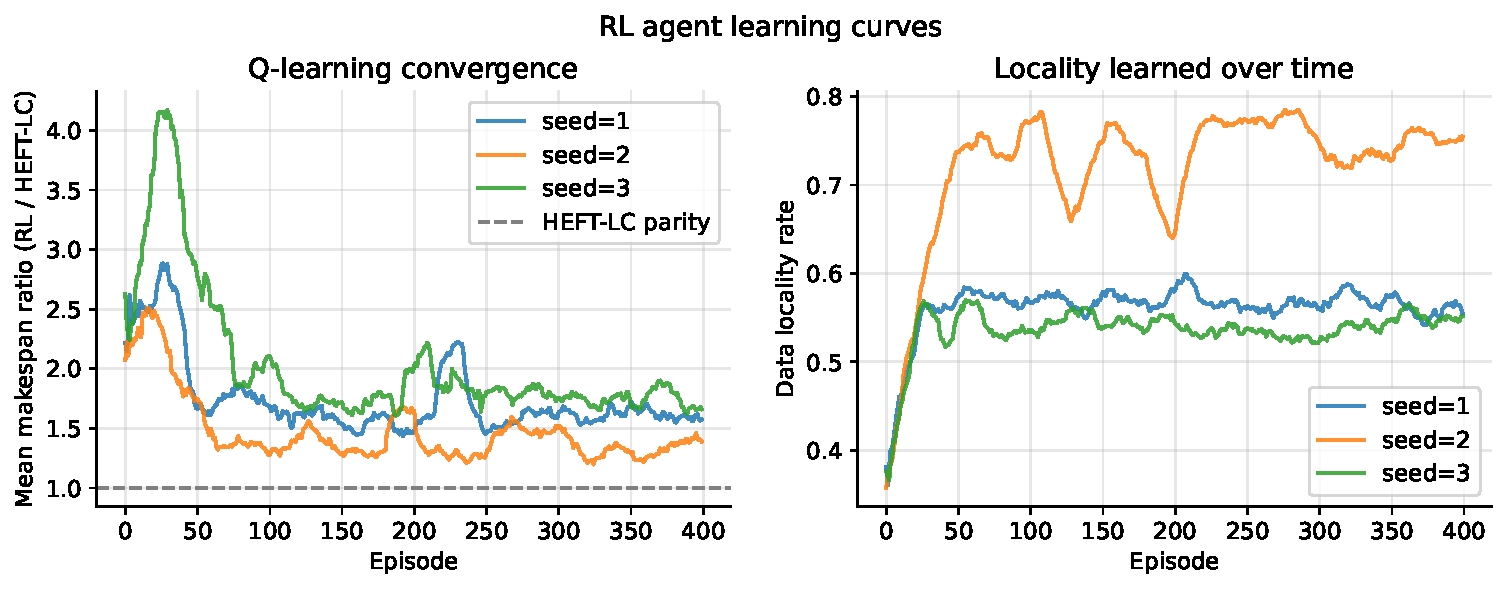
\includegraphics[width=\columnwidth]{../figures/fig5_rl_learning_curve.pdf}
\caption{Q-learning convergence (RL/HEFT-LC makespan ratio, smoothed window 20).}
\label{fig:fig5}
\end{figure}

\subsection{Makespan / imbalance trade-off}
Figure~\ref{fig:fig6} plots every run as a point in the
(imbalance, makespan) plane. The three schedulers occupy distinct regions:
HEFT-LC is tight against the left axis (best balance), DLS sits in the
lower-right (best makespan, worst balance), RL spans both directions with
high variance. No single algorithm dominates --- the operator picks the
trade-off, and the autonomic controller slides the operating point along
the HEFT-LC arc by adjusting \(\varepsilon\).

\begin{figure}[t]
\centering
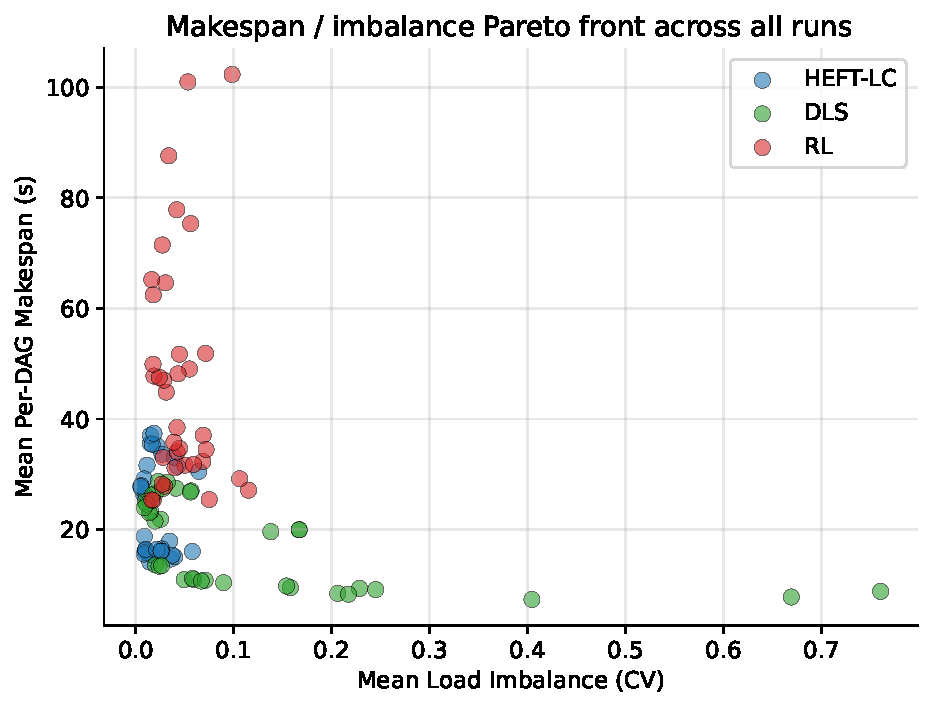
\includegraphics[width=\columnwidth]{../figures/fig6_pareto.pdf}
\caption{Makespan vs.\ imbalance: per-run scatter across scenarios.}
\label{fig:fig6}
\end{figure}

\section{Discussion}\label{sec:limits}

\textbf{When DLS wins.} DLS is dominant whenever the input-partition size
exceeds a few hundred MB and the cluster has heterogeneous bandwidth.
For small datasets (\(<100\)~MB) the locality bonus is dwarfed by the EFT
gain from picking a faster node, and HEFT-LC ties or beats it.

\textbf{When the autonomic controller helps.} The controller's value is
greatest when the literature-default \(\varepsilon = 0.05\) is wrong for
the workload at hand, which we observe both on stable streams over
heterogeneous clusters (Scenario D, 39\% makespan reduction on
\texttt{skewed\_8}) and on non-stationary streams (Scenario F, 31\%
reduction). When the default happens to be a good fit --- e.g.\ a
homogeneous cluster under modest contention --- the controller's gain
shrinks to under 15\%. In no scenario did the controller harm makespan
beyond the noise floor: the cooldown and bounded \(\varepsilon\)-step
prevent oscillation.

\textbf{Limits of tabular RL.} Our discrete state (36 cells) is too coarse
to express the local EFT landscape. The agent learns useful coarse
heuristics (preferring local nodes when load is balanced, preferring fast
nodes when not) but cannot match HEFT-LC's exact EFT comparison. Deep RL
with a continuous state \(\in \mathbb{R}^{O(n)}\) and a policy network
\cite{mao2019decima} would lift this ceiling at the cost of training time
and pre-deployment dataset requirements.

\textbf{Failure recovery.} Our failure model marks nodes unavailable but
does not re-execute interrupted tasks. A production scheduler must handle
task replay; this is orthogonal to the placement policy studied here.

\section{Related work}

HEFT \cite{topcuoglu2002} and CPOP \cite{topcuoglu2002} remain the
canonical static heuristics. PEFT \cite{arabnejad2014peft} improves HEFT by
estimating downstream cost more accurately; our work is orthogonal --- it
keeps the HEFT family intact and adds an outer adaptation loop. Decima
\cite{mao2019decima} demonstrated that GNN-based deep RL can beat
hand-tuned scheduling on Spark; our results suggest the gap between
tabular and deep RL is substantial and aligns with their findings.
On the autonomic side, Kephart \& Chess's vision paper
\cite{kephart2003vision} introduced MAPE-K; recent surveys
\cite{macias2018survey} document its application to cloud orchestration.

\section{Conclusion and future work}\label{sec:future}

We presented AdaptiveFlow, an end-to-end framework for streaming data
workflows that augments the HEFT-LC static scheduler with (i) a locality
bonus, (ii) a MAPE-K controller that self-tunes \(\varepsilon\), and
(iii) a tabular Q-learning agent. The key empirical findings are:
DLS reduces makespan by 26\% on heterogeneous-bandwidth clusters by
exploiting data locality; the autonomic controller reduces mean
makespan by 31--39\% over the static HEFT-LC default by discovering
workload-specific \(\varepsilon\) values online; and the RL agent
converges from 2.6\(\times\) to 1.6\(\times\) the HEFT-LC baseline
without surpassing it, motivating a deep-RL extension.
Three follow-up directions stand out:
(a) replace the tabular Q-learner with a small policy network using
features from the EFT vector itself; (b) extend the MAPE-K controller to
adapt the DLS locality weight \(\alpha\) jointly with \(\varepsilon\);
(c) integrate task-level fault recovery so makespan and throughput
co-degrade gracefully under heavy failure.

\section*{Reproducibility}
All code, raw CSVs, and figures are available at
\url{https://github.com/Sid00011/AdaptiveFlow}. The full benchmark runs in
under three minutes on a laptop CPU; \texttt{python experiments/run\_experiments.py}
regenerates \texttt{data/results.csv} and the auxiliary traces.

\begin{thebibliography}{9}
\bibitem{topcuoglu2002}
H.~Topcuoglu, S.~Hariri, and M.-Y.~Wu, ``Performance-Effective and
Low-Complexity Task Scheduling for Heterogeneous Computing,'' \emph{IEEE
Transactions on Parallel and Distributed Systems}, vol.~13, no.~3, pp.
260--274, 2002.

\bibitem{ullman1975np}
J.~D.~Ullman, ``NP-Complete Scheduling Problems,'' \emph{Journal of
Computer and System Sciences}, vol.~10, no.~3, pp.~384--393, 1975.

\bibitem{arabnejad2014peft}
H.~Arabnejad and J.~G.~Barbosa, ``List scheduling algorithm for
heterogeneous systems by an optimistic cost table,'' \emph{IEEE TPDS},
vol.~25, no.~3, pp.~682--694, 2014.

\bibitem{kephart2003vision}
J.~O.~Kephart and D.~M.~Chess, ``The vision of autonomic computing,''
\emph{Computer}, vol.~36, no.~1, pp.~41--50, 2003.

\bibitem{mao2019decima}
H.~Mao, M.~Schwarzkopf, S.~B.~Venkatakrishnan, Z.~Meng, and M.~Alizadeh,
``Learning Scheduling Algorithms for Data Processing Clusters,'' in
\emph{ACM SIGCOMM}, 2019.

\bibitem{macias2018survey}
M.~Macias, J.~Guitart, et al., ``A survey on self-adaptive systems for
cloud computing,'' \emph{Cluster Computing}, vol.~21, pp.~1431--1454, 2018.

\bibitem{spark}
M.~Zaharia, M.~Chowdhury, T.~Das, et al., ``Resilient Distributed Datasets:
A Fault-Tolerant Abstraction for In-Memory Cluster Computing,'' in
\emph{NSDI}, 2012.

\bibitem{kubernetes}
B.~Burns, B.~Grant, D.~Oppenheimer, E.~Brewer, and J.~Wilkes, ``Borg,
Omega, and Kubernetes,'' \emph{Comm. ACM}, vol.~59, no.~5, pp.~50--57, 2016.
\end{thebibliography}

\end{document}
